\chapter{Analysis of word embeddings}
TODO

\section{Empirical setup}
TODO: Explain what PC we are using, CPU, RAM, GPU, etc, for all experiments.

\section{Training and evaluating our word2vec implementation}
\label{sec:training-and-eval-our-word2vec-impl}
We train and evaluate our word2vec implementation to further deepen our understanding in how to implement it in practice and how it might perform versus other implementations of word2vec. As with training any machine learning model, one usually needs to prepare some data. In our case it is not any different, and before training our word2vec model, we will in this section first go over the data preprocessing choices we have made. Furthermore, we discuss the details of our own implementation of word2vec using the Skip-gram model and negative sampling. At last we cover the specific choices of hyperparameters and compare our empirical results to results from other models.

\subsection{Data preprocessing}
\label{sec:data-preprocessing}
To train a word2vec model, one needs to have a sufficiently large dataset (and thus embedding dimensionality) to yield good quality word embeddings \cite{mikolov2013b}. In the empirical experiments of \cite{mikolov2013b}, they used an internal data set from Google News. Since this dataset is not publicly available, we instead used dumps from \cite{WikimediaDumps} and performed a number of preprocessing steps, before training on it. The dumps from Wikipedia were first downloaded and parsed using the WikiExtractor tool \cite{Wikiextractor2015}. Furthermore, we created a script using Python \cite{python3-2009} to merge and process output files from the WikiExtractor tool into a certain number of text files (in our case, equal to the number of cores, to benefit from parallel reading), such that we can train on it with ease.

We then proceed by processing each Wikipedia article. In particular, we performed the following steps
\begin{enumerate}
    \item We split each article into a list of sentences using the \textit{tokenize.sent\_tokenize} function from the NLTK library \cite{bird2009natural}.
    \item Then, we preprocess each sentence individually.
    \begin{enumerate}
        \item We first replace contractions in each sentence (e.g. I'll $\mapsto$ I will, you'd $\mapsto$ you would, etc.) by using the contractions pip-package \cite{contractions-2016}.
        \item Then we split the sentence into a list of words using the \textit{word\_tokenize} function from NLTK.
        \begin{enumerate}
            \item We convert each word in the sentence to its lower-case representation.
            \item We remove punctuation from words and create new sub-words for each word delimited by punctuation (e.g. out-of-the-box $\mapsto$ out, of, the, box).
            \item At last, we replace all numbers (including ordinal numbers) with its textual representation. For example, the number 10 becomes "ten" and the word "21st" becomes "twenty-first".
        \end{enumerate}
    \end{enumerate}
    \item With the new processed sentences, we filter out sentences that have less than \textbf{min\_word\_count} words in them.
    \item Each sentence is then appended to an output text file, separated using the newline character (i.e. \textbackslash n).
\end{enumerate}

Following, we combined words that appear frequently together, such as "New York" or "programming languages", into a single word, separated by an underscore. This preprocessing procedure is explained in \cite[4 Learning Phrases]{mikolov2013b} and consists of a simple, yet efficient data-driven approach where we combine phrases together based on word counts, as shown in \cref{eqn:word2phrase-score}. This phrase-learning procedure is referred to as word2phrase, as specified by the original source code.
\begin{align}
    \label{eqn:word2phrase-score}
    \text{score}(w_i, w_j) = \frac{\text{freq}(w_i, w_j) - \delta}{\text{freq}(w_i) \cdot \text{freq}(w_j)}
\end{align}
where $w_i$ and $w_j$ are bigrams, or two neighboring words, from the vocabulary, $freq()$ returns the how many times the word (or bigram) occurs in the vocabulary and $\delta$ is a hyperparameter used to prevent long phrases consisting of infrequent words. If the score in \cref{eqn:word2phrase-score} is above the $\delta$ threshold parameter, the bigram is accepted into the vocabulary and replaces all occurrences of the two words $w_i$ and $w_j$ where they are next to each other. We denote the threshold parameter as \textbf{threshold-word2phrase}. One usually runs a couple of passes through the text data to create trigrams, four-grams or even five-grams, depending on the application at hand, and is chosen as a hyperparameter as well. We denote the number of passes through the text as \textbf{num-epochs-word2phrase}. For each pass through the data, the $\delta$ hyperparameter is decreased, but \cite{mikolov2013b} does not state how they decrease it. By manual inspection of the source code of word2vec, we observed that they started with a threshold of 200, then decreased it to 100 for the second and final pass. With this in mind, we introduce a threshold decay parameter, denoted \textbf{threshold-decay-word2phrase}, which tells how much the threshold should be decreased for each pass.

\subsection{Implementation specifics}
To implement the word2vec model, we used Python and Tensorflow \cite{python3-2009, tensorflow2015-whitepaper}. In particular, we implemented the Skip-gram model using negative sampling. To do so, we split our implementation into three main Python classes. The first class is the \path{Tokenizer}. It is responsible for converting text into word indices in vocabulary (e.g. the word "hello" $\mapsto$ 42). The second class is the \path{Word2vecSGNSModel}, which inherits the \path{tf.keras.Model} class from Tensorflow\footnote{We created the model using subclassing, as specified in \href{https://www.tensorflow.org/guide/keras/custom_layers_and_models}{this guide from Tensorflow}.}, and is the model we use to train our ANN. The third and final main class is \path{Word2vec}. It performs training using the \path{Word2vecSGNSModel} and uses \path{Tokenizer} internally to convert words into integers.

To load the data into the model, we use the \path{tf.data} API, as introduced in Tensorflow 2. The \path{tf.data} API allows us to create flexible and scalable data generators. As mentioned in \cref{sec:data-preprocessing}, we want to train our model on dumps from Wikipedia, i.e., several gigabytes of raw text data, and the \path{tf.data} API allows us to exactly this in a quick and efficient manner. In particular, we used the \path{tf.data.TextLineDataset} class to load multiple text files in parallel and set \path{num_parallel_calls} to \path{tf.data.experimental.AUTOTUNE} wherever we could, such that we parallelize the data generation process as much as possible. We also used \path{prefetch} to prepare the data on the CPU while training.

We implemented word2phrase using Python. First, we counted the uni- and bigram word occurrences, and using them, we ran the word2phrase procedure as explained in \cref{sec:data-preprocessing} by accepting bigrams into the vocabulary if the score (from \cref{eqn:word2phrase-score}) is greater than the set threshold parameter.

By implementing word2vec ourselves, we learned a few things we did not realize after reading the two original papers from Mikolov et al. \cite{mikolov2013a, mikolov2013b}
\begin{itemize}
    \item Training on big datasets (e.g. dumps from Wikipedia) requires an efficient implementation of the data generator. We first attempted to create a data generator which loaded everything into memory, but it became clear to us that this does not scale well when we later want to test on bigger data sets.
    \item Preprocessing of data may drastically change the quality of the word embeddings.
    \item There are two embedding matrices $W$ and $W'$ corresponding to the input and output of the network. At first, we only had a single embedding matrix, for both the input and the output of the network.
\end{itemize}

\subsection{Hyperparameter choices}
\label{sec:hyperparameter-choices}
To train the word2vec model, we base our choices of hyperparameters to the different choices used in models from \cite{mikolov2013a, mikolov2013b}. These hyperparameters can be found in \cref{table:word2vec-hyperparameter-choices}.

\begin{table}[ht]
    \centering
    \begin{tabular}{@{}ll@{}}
    \toprule
    Hyperparameter & Value\\
    \midrule
    \rowcolor[HTML]{F5F5F5} \textbf{min-word-count} & 5\\
    \textbf{max-vocab-size} & $\infty$ \\
    \rowcolor[HTML]{F5F5F5} \textbf{batch-size} & 256\\
    \textbf{num-epochs} & 5\\
    \rowcolor[HTML]{F5F5F5} \textbf{num-epochs-word2phrase} & 2\\
    \textbf{threshold-word2phrase} & 200\\
    \rowcolor[HTML]{F5F5F5} \textbf{threshold-decay-word2phrase} & 0.5\\
    \textbf{learning-rate} & 0.025\\
    \rowcolor[HTML]{F5F5F5} \textbf{min-learning-rate} & 0.0000025\\
    \textbf{embedding-dim} & 300\\
    \rowcolor[HTML]{F5F5F5} \textbf{max-window-size} & 5\\
    \textbf{num-negative-samples} & 5\\
    \rowcolor[HTML]{F5F5F5} \textbf{sampling-factor} & 0.00001\\
    \textbf{unigram-exponent} & 0.75\\
    \bottomrule
    \end{tabular}
    \caption{Hyperparameters used to train our word2vec model}
    \label{table:word2vec-hyperparameter-choices}
\end{table}

Similar to \cite{mikolov2013b}, we set the minimum word count to 5, i.e., we discard words that occur less than 5 times in the data we train on. In addition to this, we did not restrict the maximum vocabulary size, e.g., we let the vocabulary include any words that occur at least 5 times.

We set the number of passes for word2phrase to 2 and the initial threshold to 200, as \cite{mikolov2013b} did in their experiments. Furthermore, we set the threshold decay to 0.5 (i.e. the threshold is halved for each pass) to use a similar setup.

Neither \cite{mikolov2013a} nor \cite{mikolov2013b} stated which batch-size they used, but by inspecting the original source code\footnote{\href{https://github.com/tmikolov/word2vec/blob/e092540633572b883e25b367938b0cca2cf3c0e7/word2vec.c/\#L542}{word2vec.c at line 542 (of the original word2vec repository)}}, we concluded that they used 1 as their batch size, i.e., performing a backward pass for every forward pass in the model. We found, however, that setting the batch size to 256 to be a nice fit for our data, leading to good quality vectors and faster training.

Mikolov et al. used 1 to 4 epochs in their experiments \cite{mikolov2013a, mikolov2013b}, and in the original source code of word2vec\footnote{\href{https://github.com/tmikolov/word2vec/blob/e092540633572b883e25b367938b0cca2cf3c0e7/word2vec.c/\#L43}{word2vec.c at line 43 (of the original word2vec repository)}}, they default to 5 epochs. For this reason, we set the number of epochs to 5.

We set the initial and minimum learning rate to 0.025 and 0.000025, respectively, as noted in \cite{mikolov2013a} and the original source code of word2vec.

Furthermore, we set the embedding dimension to 300, the maximal window size to 5, the number of negative samples to 5, the sampling factor to 0.00001 and the unigram exponent to 0.75, similar to experiments from \cite{mikolov2013b}.

Using the preprocessing steps from \cref{sec:data-preprocessing} on our data and the hyperparameters from \cref{table:word2vec-hyperparameter-choices}, we get a vocabulary size of 1682564 ($\sim$1.7M) and corpus size of 2514127336 ($\sim$2.5B).

\subsection{Empirical results}
We evaluated a word2vec model trained on the hyperparameters from \cref{sec:hyperparameter-choices} on a machine with a single GPU (GeForce RTX 2080 Ti), one CPU (Intel i9-7900X @ 3.30GHz) and 64 GB of RAM. We evaluated the trained model using the SSWR and MSR test datasets and compare the results to models from \cite{mikolov2013a, mikolov2013b, mikolov-etal-2013-linguistic, bojanowski2017enriching}. In particular, we compare to the Skip-gram models from \cite[Table 3]{mikolov2013a} and \cite[Table 6]{mikolov2013a} (denoted SG 300 and 1000 respectively), the NEG-15 model from \cite[Table 1]{mikolov2013b}, the RNN-1600 model from \cite[Table 2]{mikolov-etal-2013-linguistic} and the fastText model from \cite[Table 2]{bojanowski2017enriching}. The results are shown in \cref{table:word2vec-eval-empirical-results} (a dash denotes that the model has not been evaluated on the particular subset/data set).

\begin{table}[ht]
    \centering
    \begin{tabular}{@{}cm{1.7cm}m{1.7cm}m{1.7cm}m{1.7cm}m{1.7cm}m{1.7cm}m{1.7cm}@{}}
    \toprule
    & \multicolumn{3}{c}{\cite[SSWR]{mikolov2013a}} & \multicolumn{4}{c}{ \cite[MSR]{mikolov-etal-2013-linguistic}} \\ \cmidrule(l){2-8} 
    \multirow{-2}{*}{Model} & Semantic Accuracy {[}\%{]} & Syntactic Accuracy {[}\%{]} & Total Accuracy {[}\%{]} & Adjectives Accuracy {[}\%{]} & Nouns Accuracy {[}\%{]} & Verbs Accuracy {[}\%{]} & Total Accuracy {[}\%{]} \\ \midrule
    \rowcolor[HTML]{F5F5F5}
    SG 300 & 55 & 59 & -- & -- & -- & -- & \textbf{56} \\
    SG 1000 & 66.1 & 65.1 & 65.6 & -- & -- & -- & -- \\
    \rowcolor[HTML]{F5F5F5}
    NEG-15 & 61 & 61 & 61 & -- & -- & -- & -- \\
    RNN-1600 & -- & -- & -- & 23.9 & 29.2 & \textbf{62.2} & 39.6 \\
    \rowcolor[HTML]{F5F5F5}
    fastText & \textbf{77.8} & \textbf{74.9} & -- & -- & -- & -- & -- \\
    Our model & 65.8 & 67.3 & \textbf{66.8} & \textbf{43.1} & \textbf{62.5} & 59.1 & \textbf{54.9} \\
    \bottomrule
    \end{tabular}
    \caption{Comparison of empirical results on the SSWR and MSR word analogies test data sets.}
    \label{table:word2vec-eval-empirical-results}
\end{table}

\textbf{TODO}: Comment on the result.

\begin{figure}[h]
   \centering
   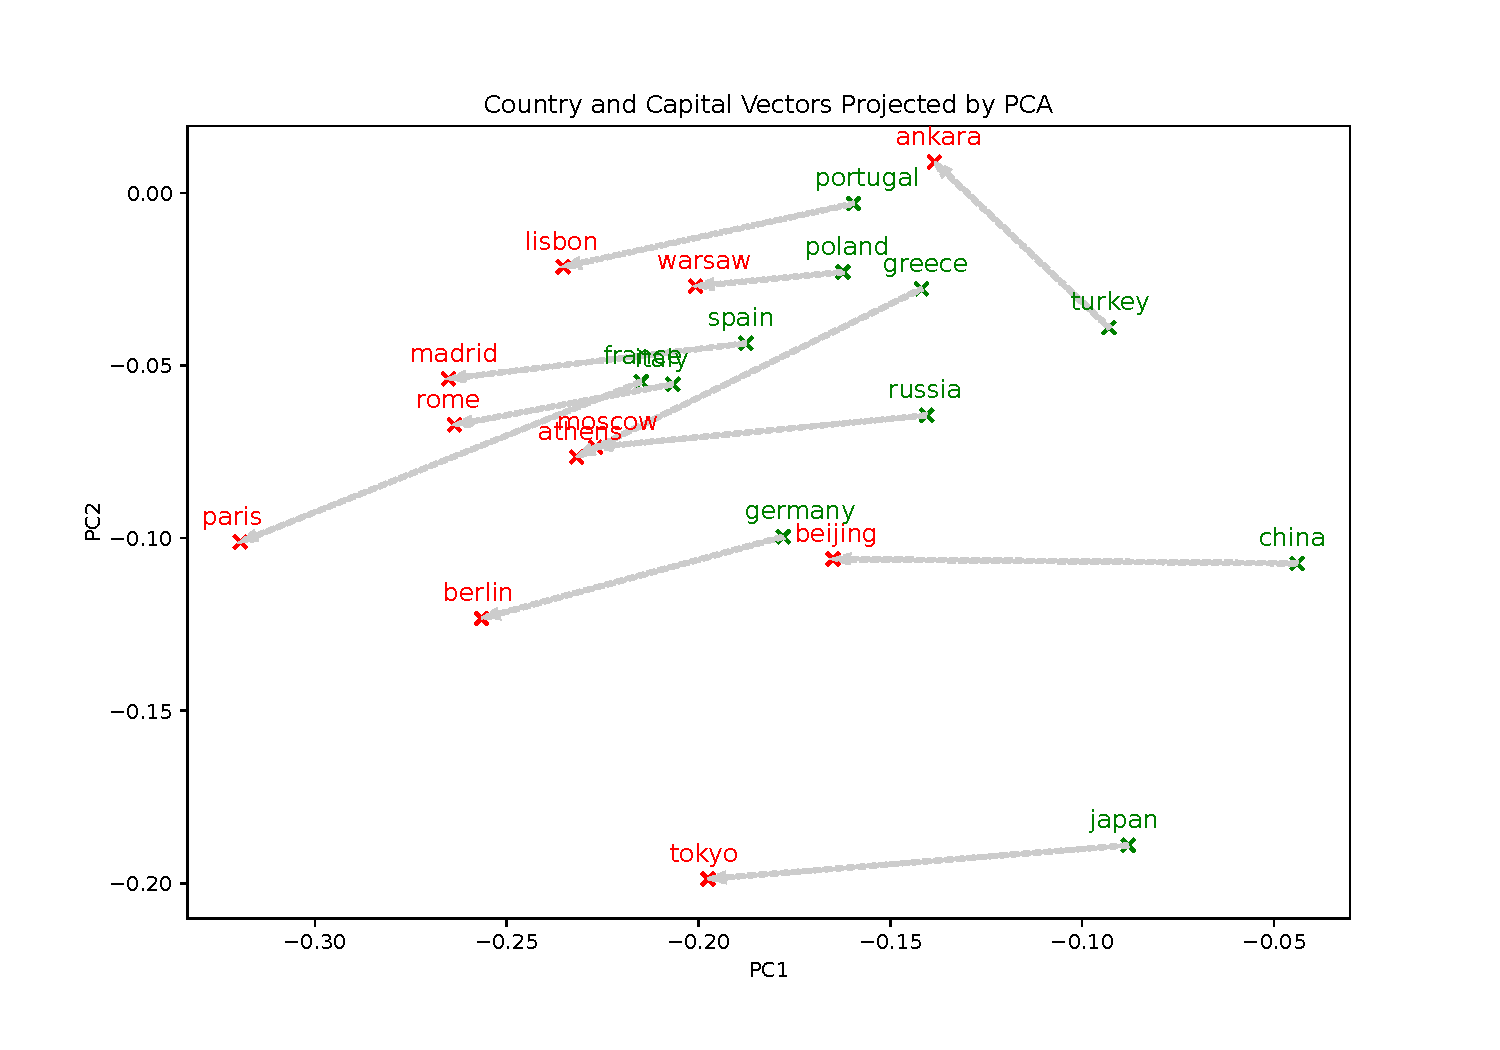
\includegraphics[width=\textwidth]{thesis/figures/country-capital-pca-2d.pdf}
 \caption{Two-dimensional PCA projection of the 300-dimensional word embeddings of some countries and their capital cities.}
 \label{fig:country-capital-pca-2d}
\end{figure}

\section{Cluster analysis}
TODO

\subsection{Comparing clustering algorithms}
TODO

\subsection{Clustering word groups}
TODO

\section{Intrinsic dimension estimation}
TODO

\section{Topological data analysis}
TODO

\subsection{Topological polysemy}
TODO

\subsection{Geoemtric anomaly detection}
TODO
